\chapter{TCE 控制器工程}

\begin{chapteroverviewbox}
本章讨论的 TCE（Temperature \& Control Executor）不是一个新的推理模型，也不是负责决定“应该完成什么任务”的规划器，更不是替代 Scheduler、CCM 或自我结构 $\Psi$ 的中央意志模块。TCE 的严格工程定位是：\textbf{在 SPC 对当前认知状态进行估计、AHC 给出连续内稳态调制背景、Scheduler 给出资源与任务包络、CCM 给出认知负载约束之后，对 Agent 当前认知动力学的增益、温度、注意范围、探索程度、搜索深度、抑制强度、记忆流速与运行节律实施连续反馈控制。}

因此，TCE 控制的不是“一个答案”，而是\textbf{产生答案、行动和记忆变化的动力学条件}。它所回答的问题不是 ``What should I think?''，而是 ``How should the cognitive system evolve now?''。如果把工作记忆 $h(t)$ 看成 Agent 当前显式认知活动的有限状态面，把 SPC 看成状态观察器，把 AHC 看成内稳态调制器，那么 TCE 就是作用于这一状态面的主要快速控制器。其工程目标是在有限工作记忆、延迟观测、环境扰动和慢结构约束下，使认知轨迹长期停留在一个可运行、可恢复、可学习的区域中，而不是追求某个瞬时变量的极大化。
\end{chapteroverviewbox}

\begin{figure}[htbp]
\centering
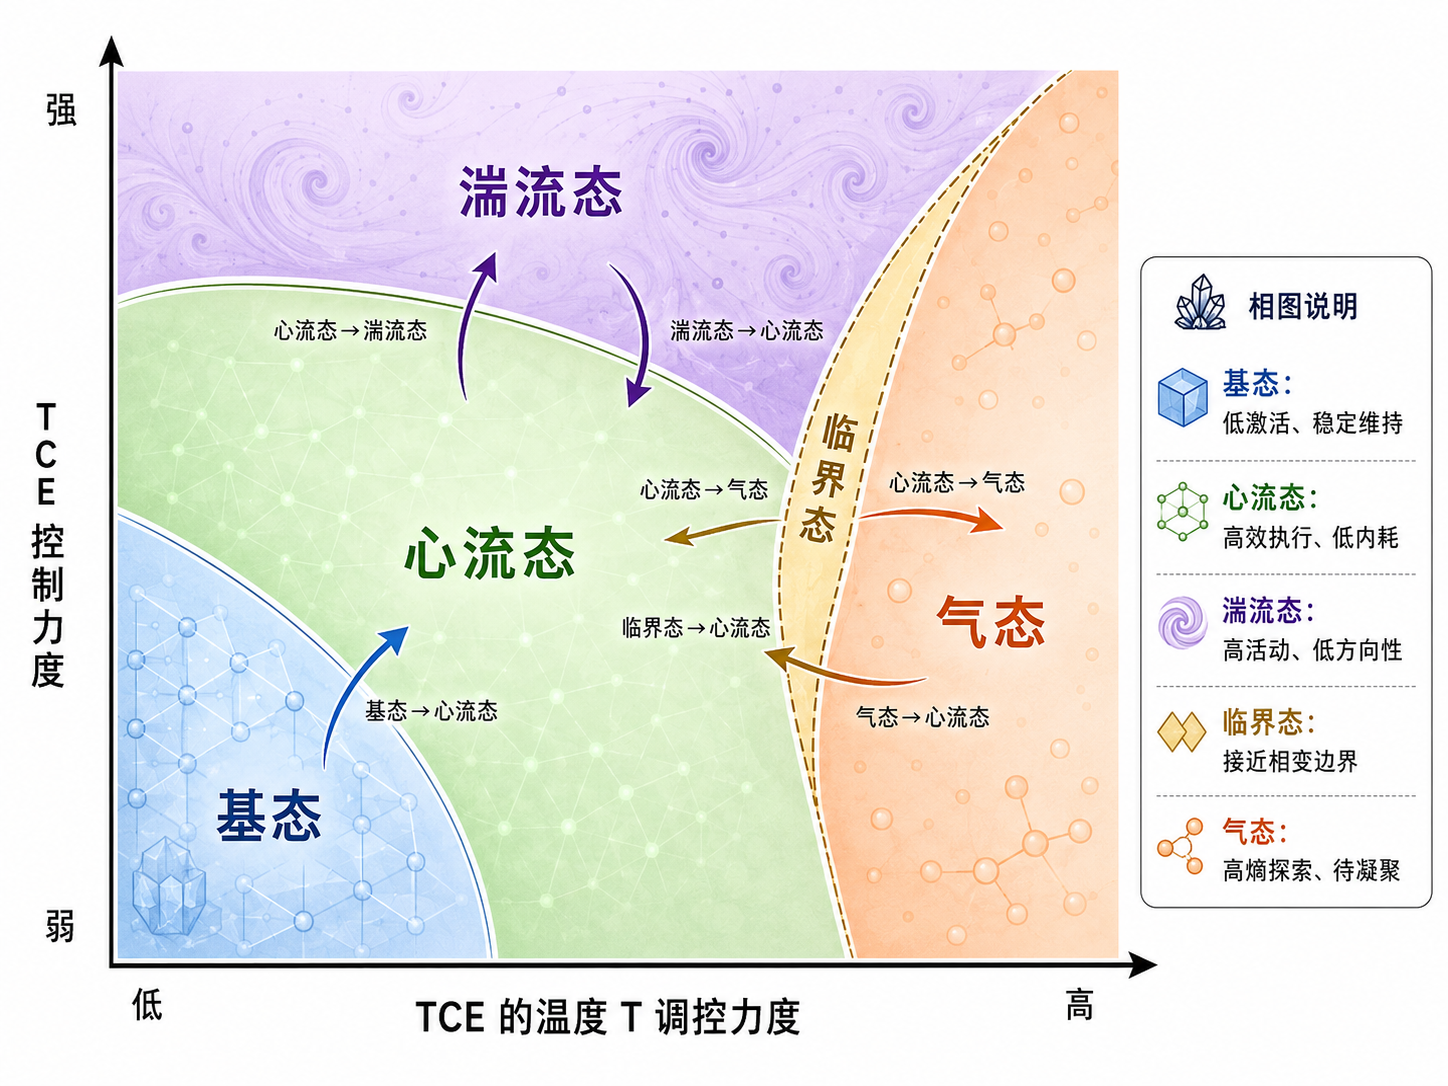
\includegraphics[width=.9\textwidth,height=.38\textheight,keepaspectratio]{images/tce-cognitive-state-phase-map.png}
\caption{TCE 控制量与运行相区域}
\end{figure}
\section{TCE 的控制对象、状态空间与统一控制向量}

前几章已经逐步建立了 AgentOS 的内部动力结构：工作记忆 $h(t)$ 承载当前被显式提升的 Agent-CSO，SPC 对工作记忆及相关内部状态进行压缩估计，AHC 将身体、资源、威胁、不确定性和社会状态积成为连续调制背景，而 Scheduler 与 CCM 分别承担任务资源配置和运行负载治理。在这个体系中，我们现在需要回答一个更加具体的控制工程问题：当系统已经知道“自己目前大致处于什么状态”，也知道“当前有哪些任务和资源约束”以后，究竟由谁改变认知活动本身的动力学形态？

这个角色就是 TCE。

我们首先把 Agent 当前与快速认知控制有关的状态抽象为

\[
x_c(t)
=
\left[
x_h(t),
a(t),
c(t),
q(t),
r(t)
\right],
\]

其中 $x_h(t)$ 表示工作记忆 $h(t)$ 的当前结构状态；$a(t)$ 表示 AHC 给出的连续调制状态；$c(t)$ 表示 CCM 所估计的运行负载和结构压力；$q(t)$ 表示当前任务、目标和调度状态；$r(t)$ 表示身体、工具和外部环境返回的相关残差信号。这里我们刻意不把 $\Psi$ 与 $\Omega$ 直接并入快速状态向量，因为它们位于远慢于 TCE 的时间尺度。它们对 TCE 的作用更接近慢约束、目标偏置和可行域塑形，而不是每一个控制周期都被 TCE 任意改变的普通状态变量。

因此，TCE 所看到的并不是 Agent 的“真实完整内部状态”，而是经过 SPC、AHC、CCM 与 Scheduler 等机制处理后的可控制状态估计：

\[
\hat x_c(t)
=
\mathcal O_{\mathrm{SPC}}
\left(
h(t),E(t),\Theta(t),a(t),c(t),q(t),r(t)
\right).
\]

这里 $\mathcal O_{\mathrm{SPC}}$ 是观察与压缩算子。由于任何状态估计都存在采样周期、推理延迟和表示误差，因此一般有

\[
\hat x_c(t)\neq x_c(t),
\]

而更合理的形式是

\[
\hat x_c(t)
=
x_c(t-\tau_o)+\epsilon_o(t),
\]

其中 $\tau_o$ 为观察延迟，$\epsilon_o(t)$ 为估计误差。这一点决定了 TCE 不可能被设计成无限高增益的瞬时纠错器；后面我们讨论过冲和振荡时会看到，这个看似简单的事实实际上决定了整个认知控制器的稳定边界。

TCE 的输出应当表示为一个多维控制向量，而不是一个所谓 ``temperature'' 标量。我们定义

\[
u_T(t)
=
\left[
T,
g,
\iota,
\alpha,
\eta,
d,
\kappa,
\nu,
\Lambda_M
\right]_t,
\]

其中：

\[
T
\]

表示认知温度，用于调节候选状态分布的平坦程度与局部确定性；

\[
g
\]

表示总体激活增益；

\[
\iota
\]

表示抑制强度；

\[
\alpha
\]

表示当前显式注意范围；

\[
\eta
\]

表示探索强度；

\[
d
\]

表示有效搜索或推理深度；

\[
\kappa
\]

表示保守度或行动前所需证据强度；

\[
\nu
\]

表示认知运行节律、更新频率或步长；

而

\[
\Lambda_M
=
\{
\lambda_{hE},
\lambda_{Eh},
\lambda_{E\Theta},
\lambda_{\Theta E},
\lambda_{\Theta h},
\ldots
\}
\]

表示与记忆流转有关的动力学速率。历史设计中，TCE 本来就不仅控制温度，还控制激活增益、抑制、认知势能以及三相记忆之间的流转速度。因此工程实现中不应把 TCE 缩减为 LLM decoding temperature 的封装。

我们可以将受控的认知动力学写成

\[
\dot x_c
=
F_c
\left(
x_c,
u_T,
u_{\mathrm{sched}},
u_{\mathrm{CCM}},
\Psi,
\Omega,
w
\right),
\]

其中 $w$ 表示外部扰动、突发事件、身体异常和新的观测残差。Scheduler 给出资源与优先级包络，CCM 给出可承载复杂度约束，而 $\Psi$ 与 $\Omega$ 定义更慢的身份、价值和生命周期方向。于是 TCE 实际上不是自由控制整个认知系统，而是在一个由其他模块共同定义的可行域中调节快速动力学：

\[
u_T(t)
\in
\mathcal U_{\mathrm{feasible}}
\left(
\Psi,
\Omega,
\mathrm{Scheduler},
\mathrm{CCM},
\mathrm{Boundary},
\mathrm{Safety}
\right).
\]

这一区分具有非常重要的工程意义。TCE 如果被允许直接改变目标、身份、价值、任务权限和身体安全约束，就会从“认知动力控制器”演化成一个缺乏边界的中央决策器，从而破坏整个 AgentOS 的分层结构。我们在本书中始终坚持：

\[
\boxed{
TCE\neq Planner,\qquad
TCE\neq Scheduler,\qquad
TCE\neq CCM,\qquad
TCE\neq \Psi.
}
\]

Planner 决定候选策略内容，Scheduler 决定谁获得资源，CCM 决定哪些认知结构可以被当前有限工作记忆承载，$\Psi$ 和 $\Omega$ 提供慢尺度的主体约束，而 TCE 决定这些活动\textbf{以怎样的动力学方式运行}。

因此，若把认知系统看成一个受控动力系统，那么本章的核心问题可以压缩为：

\[
\boxed{
\hat x_c(t)
\xrightarrow{\mathrm{TCE}}
u_T(t)
\xrightarrow{F_c}
x_c(t+\Delta t)
\xrightarrow{\mathrm{SPC}}
\hat x_c(t+\Delta t)
}
\]

这就是 TCE 控制器工程的基本闭环。

\section{控制增益：认知状态应当被改变多强}

控制增益是 TCE 工程中最容易被忽略、却又最容易引起系统性故障的变量。许多认知系统设计习惯于把控制写成一系列离散规则，例如“如果过载就降低温度”“如果不确定就增加搜索”“如果冲突就扩大注意”。这些规则在静态测试中可能有效，但对于一个长期运行的 Agent，它们仍然缺少最重要的信息：\textbf{应该改变多少？改变多快？改变之后应当等待多久再继续修正？}

这正是控制增益需要回答的问题。

设 SPC 得到的当前认知状态指标为

\[
y(t)
=
\begin{bmatrix}
C_h(t)\\
U(t)\\
R(t)\\
S(t)
\end{bmatrix},
\]

其中 $C_h$ 表示工作记忆有效负载，$U$ 表示不确定性，$R$ 表示预测或行动残差，$S$ 表示稳定性指标。设 TCE 当前希望维持的运行参考区域为

\[
y^\star(t).
\]

则定义认知状态误差

\[
e(t)=y^\star(t)-y(t).
\]

最简单的 TCE 控制器可以具有比例形式：

\[
u_T(t)
=
u_0
+
K_P e(t),
\]

其中 $K_P$ 是一个多变量增益矩阵。它不只是一个数，因为不同类型误差应该影响不同控制变量。例如工作记忆负载上升可能主要增加抑制、缩小注意范围并降低新支线准入；预测残差升高则可能扩大注意范围、提高探索并允许更多候选结构进入 h；而身体威胁升高时，系统可能同时降低搜索深度并提高行动保守度。

因此实际的增益矩阵可以写成

\[
K_P=
\begin{bmatrix}
\frac{\partial T}{\partial C_h} &
\frac{\partial T}{\partial U} &
\frac{\partial T}{\partial R} &
\frac{\partial T}{\partial S}
\\
\frac{\partial g}{\partial C_h} &
\frac{\partial g}{\partial U} &
\frac{\partial g}{\partial R} &
\frac{\partial g}{\partial S}
\\
\vdots & \vdots & \vdots & \vdots
\end{bmatrix}.
\]

这一表达提醒我们：TCE 并不是一些彼此独立的 knob，而是一个多输入多输出控制系统。改变一个输入变量往往同时改变多个认知动力学参数，多个 TCE 控制量之间也会发生耦合。

例如，单纯提高激活增益 $g$ 可能帮助系统更快聚焦于当前目标，但同时也可能增加某些局部结构的自强化，使竞争分支难以进入；提高抑制 $\iota$ 可以降低工作记忆负载，却可能造成关键弱信号被错误清除；提高温度 $T$ 可能扩大搜索，又可能增加 h 中的候选结构数量；扩大注意范围 $\alpha$ 可以获得更多外部证据，却又提高 CCM 所面对的结构负载。由此可见：

\begin{remark}
TCE 的每个控制动作几乎都存在收益—负担双重效应。
\end{remark}

因此，控制增益不宜固定。更现实的是建立 gain scheduling：

\[
K_T
=
K_T
\left(
\phi(t),
a(t),
C_h(t),
R(t),
q(t)
\right),
\]

其中 $\phi(t)$ 表示当前认知运行相态。基态、心流态、临界态和湍流态对相同误差应有完全不同的控制敏感度。例如在稳定心流态中，即便观察到短暂残差，也不应进行大幅控制；否则 TCE 自身会破坏已经形成的高效局部闭环。而在临界态附近，即便相同幅度的残差，也可能意味着系统即将越过可运行边界，此时增益应该增大。

因此可以引入相态依赖增益：

\[
K_T^{(\phi)}
=
\begin{cases}
K_G, & \phi=\mathrm{Ground},\\
K_F, & \phi=\mathrm{Flow},\\
K_C, & \phi=\mathrm{Critical},\\
K_T, & \phi=\mathrm{Turbulent},\\
K_{\mathrm{rec}}, & \phi=\mathrm{Gas/Recovery}.
\end{cases}
\]

通常我们希望满足类似

\[
\|K_F\|
<
\|K_C\|,
\]

因为 Flow 状态应尽可能少受外部调节，而 Critical 状态则允许更积极的纠偏。

在更完整的 TCE 中还可以引入积分项：

\[
u_T(t)
=
u_0+
K_Pe(t)
+
K_I\int_{t_0}^{t}e(\tau)d\tau,
\]

其意义是：一个非常小但长期持续的失配不应该永远因为未超过瞬时阈值而被忽视。例如某个任务长期处于略高于正常水平的认知负载，如果只使用瞬时阈值，系统可能一直“勉强可运行”；积分项则逐渐积累这种长期压力，最终触发负载压缩、任务拆分或更慢层级的结构调整。

但认知控制中的积分项必须谨慎，因为它容易发生 windup。当外部约束使某一目标暂时无法达到时，积分误差仍不断积累，等约束解除之后就可能导致巨大的反向控制。因此可以定义：

\[
I(t)
=
\mathrm{clip}
\left(
I(t-\Delta t)+e(t)\Delta t,
I_{\min},
I_{\max}
\right).
\]

这一看似普通的控制技巧，在 AgentOS 中具有重要意义：一个长期未解决的问题，不应该无限积累成越来越高的内部“控制压力”。否则 TCE 可能逐渐把整个认知系统都围绕一个当前不可解决目标组织起来。

因此，本节最重要的结论不是“增益应高还是低”，而是：

\begin{conclusion}
TCE 必须控制认知控制本身的强度。
\end{conclusion}

一个成熟 Agent 不是时时被中央控制器紧紧握住，而应在局部结构能够自行闭合时降低高层增益，在持续残差或接近失稳边界时才增加控制强度。这与全书此前反复形成的原则一致：

\[
\boxed{
SlowGovernance\neq FastMicromanagement.
}
\]

TCE 的成熟并不是控制得越来越多，而是越来越准确地知道什么时候应该少控制，什么时候必须强控制。

\section{认知温度：候选结构分布的可塑性控制}

“温度”是 TCE 名称中最早存在的变量，但也是最容易被误解的变量。若我们把 TCE 的 Temperature 简单等价于语言模型生成中的 sampling temperature，那么整个 TCE 理论就会退化成一个极窄的 decoding 参数控制器。事实上，在 AgentOS 中，认知温度描述的是更一般的动力学性质：\textbf{当前认知状态在候选 Agent-CSO、解释、策略和未来轨迹之间进行迁移的容易程度。}

设当前工作记忆存在一组可被激活的候选认知状态

\[
\mathcal Z
=
\{z_1,z_2,\ldots,z_n\},
\]

每个候选状态具有一个当前有效势能或代价

\[
V_i
=
V(z_i\mid h,E,\Theta,\Psi,\Omega,a).
\]

可以用类似 Gibbs 分布的形式描述候选状态占据概率：

\[
p_i(T)
=
\frac{
\exp\left[-V_i/T\right]
}{
\sum_j
\exp\left[-V_j/T\right]
}.
\]

这里不应把这一公式理解成 Agent 真实神经动力学必须服从热力学，而应把它作为一种控制形式化：$T$ 越小，系统越集中于当前低代价候选；$T$ 越大，不同候选之间的概率差异越小。

因此：

\[
T\downarrow
\Rightarrow
\text{Convergence}\uparrow,
\]

而：

\[
T\uparrow
\Rightarrow
\text{Exploration}\uparrow.
\]

但是温度和探索并不完全相同。探索 $\eta$ 更接近策略级“是否主动访问新的候选域”，而温度 $T$ 更接近状态分布本身的平坦程度。一个系统可以具有较高温度但很窄的注意范围，此时只是在一个小局部中频繁跳动；也可以具有中等温度但很强的主动探索，此时它会有策略地访问多个新的结构区域。因此工程实现必须把 $T$ 与 $\eta$ 分开。

我们还可以定义工作记忆候选分布熵：

\[
H_h(T)
=
-
\sum_i p_i(T)\log p_i(T).
\]

一般而言，

\[
\frac{\partial H_h}{\partial T}>0,
\]

即温度越高，候选分布越分散。但 AgentOS 的目标并不是最大化或最小化该熵，而是让候选多样性与任务阶段相匹配。

例如在问题刚进入 h 时，系统可能处于高不确定性状态：

\[
U(t)\gg U_{\mathrm{nominal}},
\]

此时 TCE 可以适当提高 $T$，允许不同解释竞争；随着证据累积和一个结构获得持续支持，应逐步降低温度：

\[
T(t+\Delta t)<T(t),
\]

使状态逐渐收敛。可以用一个目标不确定度控制形式表示：

\[
\dot T
=
k_T
\left[
U(t)-U^\star(q(t))
\right]
-
k_R R_{\mathrm{osc}}(t),
\]

其中 $U^\star$ 是与任务阶段相关的合理不确定性目标，而 $R_{\mathrm{osc}}$ 表示已经出现的状态切换频率或振荡风险。这样可以避免“不确定越高就无限升温”。

温度还应受到 AHC 的调制。例如高 Threat 状态下，如果仍然提高开放探索程度，可能造成危险情况下的迟滞。因此可以定义：

\[
T_{\mathrm{eff}}
=
T_{\mathrm{cog}}
\cdot
m_{\mathrm{AHC}},
\]

其中：

\[
0<m_{\mathrm{AHC}}\le 1
\]

可以在高风险状态中压低实际探索温度。但需要特别注意：AHC 不应该简单地“威胁越高，温度越低”。在某些异常环境中，过度确定反而危险。若当前策略不断失败：

\[
R(t)\uparrow,
\]

那么即使 Threat 较高，也必须允许有限程度的策略逃逸。因此更合理的是：

\[
T_{\mathrm{eff}}
=
f(
U,
R,
Threat,
Urgency,
CapabilityMargin
).
\]

这实际上揭示了 TCE 的一个基本思想：认知温度不只是“随机度”，而是\textbf{结构可塑性速率的控制量}。

太低的温度会造成：

\begin{statementbox}
PrematureCollapse
\end{statementbox}

即系统过早锁定一个假设、策略或世界解释。

太高的温度会造成：

\begin{statementbox}
PersistentDispersion
\end{statementbox}

即 Agent 无法形成稳定计划，工作记忆中大量候选长期竞争。

从 h 的运行相态看，温度轴与我们此前提出的认知相图直接相关。非常低温可能造成僵化，适中温度与合理控制强度可以形成 Ground 或 Flow，而高温配合过宽注意范围和过弱抑制则可能进入 Turbulent，进一步失去结构约束时甚至进入 Gas-like 状态。

因此，本章对 Temperature 的严格定义可以写成：

\[
\boxed{
T
=
\text{TCE 对当前认知状态在可行候选结构之间迁移自由度的控制变量。}
}
\]

它既不是随机噪声，也不是智慧程度，而是 Agent 在“稳定已有结构”与“允许结构重新组织”之间进行实时调节的一个关键控制维度。

\section{注意控制：决定有限工作记忆承载哪一部分世界}

如果工作记忆容量有限，那么注意控制就不是附加功能，而是整个 AgentOS 必然存在的资源分配机制。我们已经在前文建立：

\[
C_h(t)\le C_{\max},
\]

因此 TCE 不可能通过“把更多东西全部放入 h”来解决不确定性。真正的工程问题是：在世界、身体、记忆、目标、工具、其他 Agent 和内部状态不断产生新信息的情况下，当前有限的显式认知面应该被谁占据？

注意控制可以表示成对 Agent-CSO 活跃集合的权重分配。设候选结构为

\[
\mathcal C_t
=
\{C_1,\ldots,C_n\},
\]

定义注意权重

\[
a_i(t)\in[0,1],
\]

满足

\[
\sum_i a_i(t)\le 1.
\]

当前显式认知负载可以近似写为

\[
C_h(t)
=
\sum_i
a_i(t)c_i(t)
+
\sum_{i,j}
a_i(t)a_j(t)r_{ij}(t),
\]

其中 $c_i$ 描述单个结构本身的承载负担，而 $r_{ij}$ 描述结构之间关系带来的额外负担。这个表达比单纯“工作记忆能放多少 item”更加接近我们的原始理论，因为真正使 h 崩溃的往往不是对象数量，而是对象之间需要同时维持的关系结构。

因此，TCE 控制注意并不是简单调整 softmax 权重，而至少要控制两个量：

\[
\alpha_t
=
|\mathcal C_t^{active}|,
\]

即注意覆盖宽度；

以及：

\[
\gamma_t,
\]

即注意集中程度。

系统可能有：

\[
\alpha\uparrow,\gamma\downarrow
\]

的广域扫描模式，也可能有：

\[
\alpha\downarrow,\gamma\uparrow
\]

的局部深度模式。

对于稳定执行型任务，我们希望：

\[
\alpha\downarrow,
\qquad
\gamma\uparrow,
\]

使 h 只承载当前行动链真正相关的少量结构。而在出现持续异常残差时，则可能需要：

\[
\alpha\uparrow,
\]

重新纳入此前被忽略的环境、身体、记忆或目标结构。

因此注意控制必须与“异常向上”原则结合：

\[
Residual\uparrow
\Rightarrow
PromotionProbability(C_i)\uparrow.
\]

一个正常情况下在 Body Runtime 内局部闭合的结构，不需要持续进入 h；只有当预测残差、风险、新颖度或目标相关性达到阈值时，它才应该被提升：

\[
\Gamma_i
=
f(
R_i,
Risk_i,
Novelty_i,
Persistence_i,
GoalRel_i
).
\]

当

\[
\Gamma_i<\theta_a,
\]

该结构保持局部；

当

\[
\Gamma_i\ge\theta_a,
\]

TCE 与 Scheduler/CCM 协同扩大其注意权重。

需要强调的是：TCE 不应该独自判断“哪个内容重要”。重要性本身受到 $\Psi$、Goal、Scheduler、Boundary 和 CCM 的共同作用。TCE 控制的主要是\textbf{当前已经被判定为候选结构以后，其激活、保持和竞争的动力学强度}。

可以写成：

\[
\dot a_i
=
g_i
\left(
Priority_i,
Residual_i,
GoalRel_i,
SelfRel_i
\right)
-
\iota_i a_i
-
\lambda_C\frac{\partial C_h}{\partial a_i}.
\]

第一项负责提升高价值结构，第二项代表抑制和自然衰减，第三项体现有限工作记忆容量产生的负反馈。

由此我们可以理解为什么成熟智能不是“注意更多”，而是：

\[
\boxed{
MatureIntelligence
=
SelectiveExplicitCognition.
}
\]

当越来越多熟练结构下沉到 $\Theta$、Skill、Body Runtime 或外部工具之后，真正需要进入 h 的内容反而应该减少。若一个 Agent 随能力增长反而需要越来越多全局注意力才能完成熟悉任务，那么从 AgentOS 理论看，这不是成熟，而是结构没有完成正确沉降。

TCE 的注意控制因此承担一个非常重要的跨尺度角色：它不是把整个世界压进 Agent 内部，而是不断调节当前“高清认知窗口”落在哪里。在具身系统中，这一原则后来还会延伸到 SGC 的局部高清输入控制；但即便暂时不涉及 Body 细节，其本质已经很清楚：

\begin{proposition*}
注意不是获得更多世界，而是在有限认知面上决定哪一部分世界当前值得被显式承载。
\end{proposition*}

\section{探索控制：什么时候允许认知离开已有结构}

温度调节的是候选状态分布的可塑程度，而探索控制决定的是系统是否应该主动离开当前熟悉结构，访问新的状态区域。二者相关，但在工程上必须严格分开。

假设 Agent 当前拥有一个由 $\Theta$ 和 E 支持的认知策略族

\[
\Pi_{\mathrm{known}}
=
\{\pi_1,\ldots,\pi_m\}.
\]

对于熟悉任务，Agent 理应优先利用这些稳定结构：

\[
\pi^\star
=
\arg\max_{\pi_i\in\Pi_{\mathrm{known}}}
\mathbb E[U(\pi_i)].
\]

但是当环境新颖、残差持续升高或者已有策略全部失效时，继续 exploit 已有结构会导致认知闭锁。于是需要引入探索控制量：

\[
\eta(t)\in[0,1].
\]

我们可以把候选动作或认知路径分布写成：

\[
\pi_T
=
(1-\eta)\pi_{\mathrm{known}}
+
\eta\pi_{\mathrm{novel}},
\]

其中 $\pi_{\mathrm{novel}}$ 不必表示随机行为，而可以是未充分验证的推理路径、记忆组合、工具策略或反事实模型。

因此，TCE 的探索控制不是简单“增加随机性”，而是决定：

\begin{statementbox}
有多少认知资源可以被用于当前结构之外的搜索。
\end{statementbox}

探索强度应至少受到五类因素影响：

\[
\eta
=
f(
Novelty,
Residual,
Uncertainty,
Risk,
ResourceMargin
).
\]

其中 Novelty 和 Residual 通常推动探索增加，而 Risk 和资源不足则限制探索规模。

例如，若系统面对一个低风险研究问题，可以允许：

\[
\eta\uparrow,
\quad
T\uparrow,
\quad
d\uparrow,
\]

进行大量结构尝试。

但若系统正在控制高速身体并接近危险边界，即便存在不确定性，也不能无限扩大探索。此时更合理的控制是：

\[
\eta\downarrow,
\qquad
\kappa\uparrow,
\]

优先使用经过验证的安全策略，并把高层探索放到模拟、反事实或离线结构中进行。

因此我们定义探索预算：

\[
B_{\mathrm{explore}}(t),
\]

并要求：

\[
Cost_{\mathrm{explore}}(t)
\le
B_{\mathrm{explore}}(t).
\]

这个预算由 Scheduler、CCM、Body risk 和 AHC 状态共同约束。

进一步地，探索不应该只是短时间反应，还要受到长期失败历史影响。设某个策略族的持续残差为：

\[
\bar R_T
=
\frac{1}{T}
\int_{t-T}^{t}R(\tau)d\tau.
\]

如果：

\[
\bar R_T>\theta_R,
\]

则即使当前瞬时状态尚未完全失败，也可以逐步提高探索：

\[
\dot\eta
=
k_\eta
(\bar R_T-\theta_R).
\]

这体现了前文反复讨论的：

\begin{statementbox}
PersistentFastResidualShapesSlowStructure.
\end{statementbox}

当然，TCE 本身仍位于较快控制层，它不能直接改变 $\Theta$ 或功能拓扑；但它可以通过改变探索资源，让新的结构组合获得进入 h、E 和后续学习过程的机会。

探索控制还必须解决一个重要的问题：何时停止探索。如果缺乏停止机制，一个系统可能陷入永远寻找“更好可能性”的状态，从而无法行动。可以定义当前最佳候选与次优候选的价值间隔：

\[
\Delta Q
=
Q_{(1)}-Q_{(2)},
\]

以及预测不确定性：

\[
U_Q.
\]

当：

\[
\Delta Q
>
\beta U_Q,
\]

并且主要风险约束已经满足时，可以降低探索：

\[
\eta\downarrow,
\]

进入收敛和执行阶段。

因此 TCE 的探索控制实际上在不断管理一个基本张力：

\[
\boxed{
Plasticity
\leftrightarrow
Commitment.
}
\]

探索太弱，系统形成僵化；探索太强，系统无法形成稳定行为。成熟 TCE 的目标不是最大化创新，而是在现实约束、任务阶段和工作记忆容量允许的范围内，维持一种\textbf{受控开放性}。

\section{搜索深度：应该把一次认知推进多远}

大语言模型推理系统中经常存在一种隐含假设：如果当前答案不够好，就增加更多推理步骤。然而在长期 AgentOS 中，“更深”并不是普遍优越。搜索深度增加会带来更多候选、更多中间变量、更长延迟以及更高的错误传播风险。因此 TCE 必须把搜索深度 $d$ 当作一个显式控制变量。

设一次认知搜索树为

\[
\mathcal T_s,
\]

平均分支因子为 $b$，深度为 $d$。若不进行剪枝，候选数大致为

\[
N(d)
\sim
\sum_{k=0}^{d}b^k
=
\frac{b^{d+1}-1}{b-1}.
\]

因此搜索负担随 $d$ 呈指数增长。即使真实 LLM 推理并不是显式树搜索，这一数学形式仍说明一个工程事实：当系统同时保留多个候选路径时，更深推理会快速占用工作记忆和计算资源。

于是 TCE 不应控制“最大允许思考长度”，而应动态决定边际搜索价值：

\[
MB(d)
=
\frac{
\partial \mathbb E[Utility]
}{
\partial d
},
\]

以及边际搜索成本：

\[
MC(d)
=
\frac{
\partial Cost
}{
\partial d
}.
\]

最合理的停止条件是：

\[
MB(d)
\le
MC(d).
\]

这里 Cost 至少包含：

\[
Cost
=
\lambda_1C_h
+
\lambda_2Latency
+
\lambda_3Compute
+
\lambda_4Risk_{\mathrm{drift}}
+
\lambda_5OpportunityCost.
\]

这意味着一个低价值问题不值得进行几十层深推理；一个高风险、高价值、不可逆任务则可能值得消耗更多时间进行验证。

因此可以把搜索深度设为：

\[
d^\star
=
\arg\max_d
\left[
\mathbb E U(d)-Cost(d)
\right].
\]

但 TCE 并不直接精确计算这一优化问题，而可以利用 SPC、Scheduler、CCM 与 AHC 提供的观测近似控制：

\[
d_{t+1}
=
d_t
+
k_1U_t
+
k_2Risk_t
+
k_3GoalValue_t
-
k_4C_h(t)
-
k_5Urgency_t.
\]

这里需要注意一个看似矛盾的情况：Risk 可以增加搜索深度，也可以减少搜索深度。区别在于风险是否允许延迟。如果任务是高风险但可等待的，例如设计一个长期工程方案，则应增加验证深度；如果是高风险且时间极短，例如身体即将碰撞，则高层搜索深度反而应立即下降，快速控制交给 Body Runtime 或安全控制器。因此更准确地应该引入时间余量：

\[
M_t
=
TimeToDeadline_t.
\]

于是：

\[
d^\star
=
f(
Risk,
Uncertainty,
GoalValue,
C_h,
M_t
).
\]

当：

\[
M_t\rightarrow0,
\]

高层认知搜索必须收缩。

另外，搜索深度与 $\Theta$ 的成熟程度也有关。若系统面对一个已经高度熟练的问题，继续展开显式搜索是一种浪费。因此可以定义结构成熟度：

\[
M_\Theta(C)\in[0,1].
\]

当：

\[
M_\Theta(C)\rightarrow1
\]

且运行残差低时：

\[
d^\star\downarrow.
\]

这正是“成熟能力向下沉降”的认知版本。高手之所以表现得快，并不意味着其内部没有结构，而是大量原本必须展开的搜索已经被压缩成稳定生成结构和技能闭环。

因此，TCE 对搜索深度的调节还具有一个评价成熟智能的重要指标：

\[
\boxed{
\frac{
\text{Explicit Search Depth}
}{
\text{Successful Task Complexity}
}
\downarrow
}
\]

往往意味着更多任务已经被结构化地掌握。

同时，我们必须避免另一种极端：在残差已经长期升高时仍然依赖 $\Theta$ 的旧结构快速处理。此时 TCE 应重新增加 $d$，使原本被自动化的认知结构重新显式化：

\[
ProceduralCSO
\rightarrow
ExplicitCSO.
\]

这就是“能力向下、异常向上”在搜索深度控制中的具体工程表现。

因此，搜索深度控制本质上不是“让 Agent 思考多久”，而是：

\begin{statementbox}
决定当前问题有多少结构必须重新进入显式因果展开。
\end{statementbox}

\section{保守度：证据、风险与行动承诺之间的控制}

TCE 的保守度 $\kappa$ 描述的是 Agent 在从认知状态进入行动、承诺或不可逆决策之前，需要多强的证据与稳定性保证。它与温度、探索和搜索深度相关，但不能由它们替代。

一个 Agent 可以处于高探索状态，却仍然对实际行动保持高度保守。例如在内部模拟中允许大量激进候选，并不意味着立刻执行其中任何一个方案。因此，保守度控制的真正对象是：

\[
\boxed{
\text{Representation}
\rightarrow
\text{Commitment}
}
\]

之间的阈值。

设当前最佳行动 $a^\star$ 的期望价值为：

\[
Q(a^\star),
\]

不确定性为：

\[
\sigma_Q(a^\star),
\]

潜在损失为：

\[
L(a^\star),
\]

可逆性为：

\[
Rev(a^\star)\in[0,1].
\]

我们可以定义一个风险调整后的行动置信度：

\[
\chi(a)
=
Q(a)
-
\kappa_1\sigma_Q(a)
-
\kappa_2L(a)
+
\kappa_3Rev(a).
\]

执行条件为：

\[
\chi(a^\star)
>
\theta_{\mathrm{act}}.
\]

TCE 的保守控制并不是直接修改 $Q$，而是调节阈值或风险权重。定义：

\[
\kappa(t)
=
f(
Threat,
Uncertainty,
Irreversibility,
Authority,
CapabilityMargin
).
\]

则高不可逆、高权限、高潜在损害的行为应满足：

\[
\kappa\uparrow.
\]

而低风险、可撤回的行为可以：

\[
\kappa\downarrow,
\]

允许快速探索和试错。

这与我们整个 AgentOS 的基本工程方向高度一致：不是给所有行为施加同一个安全阈值，而是根据行动后果和恢复能力建立分层控制。

特别重要的是，保守度还受到 Agent 当前能力边界的影响。设 Body Runtime 或相关 Skill 给出的 capability margin 为：

\[
M_{\mathrm{cap}}.
\]

如果：

\[
M_{\mathrm{cap}}\downarrow,
\]

即系统当前接近能力边界，则即使认知层认为某一行动具有较高期望收益，TCE 仍应增加 $\kappa$。这使“我认为值得做”和“我当前有能力安全地做”在控制上被明确区分。

保守度还应该受到 $\Psi$ 和 $\Omega$ 的慢约束。某些行为虽然短期收益很高，却严重偏离长期身份或生命周期方向，那么它们的有效阈值应提高：

\[
\kappa_{\mathrm{eff}}
=
\kappa_0
+
\lambda_\Psi
D_\Psi(a)
+
\lambda_\Omega
D_\Omega(a),
\]

其中 $D_\Psi$ 和 $D_\Omega$ 表示行动与慢结构的一致性距离。

这里我们必须特别避免一种错误实现：让 TCE 自己重新定义 $\Psi$ 或 $\Omega$ 来降低行动门槛。TCE 只能读取慢结构约束，而不能为了快速完成当前任务去修改约束本身。这就是多时间尺度系统中的 Slow Variable Protection。

在工作记忆相态层面，不同相态还应拥有不同保守策略。在 Flow 状态下，系统可能拥有较高局部能力置信度，因此在已经熟练的领域中可以降低不必要的显式确认；而在 Turbulent 或 Critical 状态下，即使系统表面上仍能生成行动计划，也应提高行动保守度：

\[
\phi\in
\{\mathrm{Critical,Turbulent}\}
\Rightarrow
\kappa\uparrow.
\]

这是因为此时问题不是某一个候选动作本身，而是 Agent 当前的内部状态估计可靠性下降。

因此，保守度并不是“胆小程度”，而是一个控制意义上的：

\begin{statementbox}
CommitmentThreshold.
\end{statementbox}

一个成熟的 Agent 既不能因保守度过高而失去现实行动能力，也不能因保守度过低而把内部未稳定的候选结构直接写入世界。

TCE 的任务是在：

\begin{statementbox}
\centering\bfseries
探索自由度
$\longleftrightarrow$
现实承诺强度
\end{statementbox}

之间建立一道动态阀门。

\section{过冲：为什么正确的调节也可能把系统推向错误状态}

到目前为止，我们一直假设 TCE 的调节方向是正确的。例如检测到负载过高就增加抑制，检测到不确定性高就增加搜索，检测到搜索过度就降低温度。但在真实控制系统中，即使控制方向完全正确，也可能因为延迟和增益过大导致过冲。

这是理解长期 Agent 心理稳定性的关键。

设认知负载状态为 $c(t)$，理想运行值为：

\[
c^\star.
\]

若 TCE 使用比例控制：

\[
u(t)
=
-k(c(t-\tau)-c^\star),
\]

而认知系统的简化动力学为：

\[
\dot c(t)
=
-ac(t)+bu(t),
\]

则有：

\[
\dot c(t)
=
-ac(t)
-
bk
\left[
c(t-\tau)-c^\star
\right].
\]

即使 $a,b,k>0$，只要 $\tau>0$ 且 $k$ 足够大，系统就可能产生过冲和振荡。

直观地说：

SPC 在 $t_0$ 时刻观察到“认知过载”。

TCE 开始强力降低激活范围。

但这一动作真正影响 h 需要时间。

在此期间 SPC 仍然继续观察到“过载”，于是 TCE 再次加强控制。

等第一轮控制效果真正显现时，后续控制已经累积，于是系统从“过载”直接越过正常区进入“过度抑制”。

随后 SPC 又观察到认知活性不足，TCE 反向增加增益。

最终形成：

\[
Overload
\rightarrow
OverSuppression
\rightarrow
UnderActivation
\rightarrow
OverExcitation
\rightarrow
Overload.
\]

这就是典型的认知过冲循环。

因此我们需要定义最大过冲量：

\[
M_p
=
\frac{
|y_{\max}-y^\star|
}{
|y(0)-y^\star|
},
\]

以及调节时间：

\[
T_s
=
\inf
\left\{
t:
|y(\tau)-y^\star|<\epsilon,
\forall\tau>t
\right\}.
\]

对于长期 Agent，TCE 的目标不是使：

\[
T_s\rightarrow0,
\]

因为极端追求快速恢复通常意味着更高增益，反而增加过冲。更合理的是在：

\[
SettlingTime
\]

和：

\[
Overshoot
\]

之间取得平衡。

可以定义代价：

\[
J_{\mathrm{reg}}
=
\int_0^\infty
\left[
e(t)^TQe(t)
+
u_T(t)^TRu_T(t)
+
\lambda_o
\|\dot u_T(t)\|^2
\right]dt.
\]

第三项特别重要，因为它惩罚 TCE 自身变化过快。也就是说，我们不仅不希望认知状态猛烈震荡，也不希望控制器不断猛烈改变控制参数。

因此可以对控制向量增加 rate limit：

\[
\|\dot u_T(t)\|
\le
r_{\max}.
\]

例如温度不能瞬间从极高跳到极低，注意范围不能每个周期大幅收缩和扩张，探索预算不能因单次异常立即翻倍。

另外，我们还需要 deadband：

\[
|e(t)|<\delta
\Rightarrow
\Delta u_T=0.
\]

其意义是：正常认知状态本来就存在波动，TCE 不应试图纠正每一点微小偏差。没有 deadband 的控制器会不断追逐噪声。

因此，对 TCE 而言一个非常重要的原则是：

\begin{statementbox}
NotEveryDeviationRequiresCorrection.
\end{statementbox}

甚至可以更进一步：

\begin{statementbox}
健康认知不是没有波动，而是波动能够在无需高层强控制的情况下自行回到可运行区域。
\end{statementbox}

这与 AgentOS 一贯强调的局部闭环和局部自治一致。

所以 TCE 对过冲的治理至少包括：

低通滤波；

变化率限制；

控制死区；

状态持续性判断；

动态增益；

积分 anti-windup；

相态依赖阈值。

最终，TCE 不应追求“即时把系统拉回某一个精确点”，而应该维持一个允许自然认知波动的可行区域：

\[
\boxed{
\mathcal R_{\mathrm{healthy}}
=
\{
x:
C_h<C_{\max},
Risk<R_{\max},
Stability>S_{\min}
\}.
}
\]

只要系统仍然处于这个区域，就不必强行微调每个变量。这实际上是从点控制转向集合控制，也是 AgentOS 控制工程与简单规则系统的重要区别。

\section{振荡：TCE 何时会成为认知不稳定性的来源}

过冲是一次控制动作越过目标区域，而振荡则意味着这种越过在反馈闭环中反复出现。当我们进入长期 Agent 控制工程时，振荡是比单次过冲更加危险的问题，因为一个反复修改自己的认知控制器可能在没有任何外部世界变化的情况下，仅凭内部 observer--controller interaction 就产生持续波动。

我们先考虑最简单的一维线性化模型。设认知状态偏差为：

\[
\delta x(t)=x(t)-x^\star.
\]

系统近似满足：

\[
\dot{\delta x}
=
A\delta x
+
Bu,
\]

TCE 控制：

\[
u=-K\hat{\delta x},
\]

而：

\[
\hat{\delta x}(t)
=
\delta x(t-\tau).
\]

于是：

\[
\dot{\delta x}(t)
=
A\delta x(t)
-
BK\delta x(t-\tau).
\]

其特征方程包含：

\[
\det
\left[
sI-A+BKe^{-s\tau}
\right]
=0.
\]

由于：

\[
e^{-s\tau}
\]

引入额外相位延迟，控制增益越高，闭环越可能跨过稳定边界。这就是为什么：

\[
Gain\uparrow
+
Delay>0
\]

会增加 oscillation risk。

在 AgentOS 中，延迟来源很多：

SPC 对 h 的状态压缩需要时间；

AHC 是积分性慢变量；

LLM 推理本身存在完成时间；

CCM 的负载策略可能并非立即生效；

Memory 写入与召回具有延迟；

Body Runtime 的现实反馈也不可能瞬时返回。

因此 TCE 不可能假设：

\[
\tau=0.
\]

更复杂的是，TCE 是多变量控制器。例如提高温度增加候选结构数量，会导致 CCM 负载升高；CCM 又要求 TCE 收缩注意；注意收缩降低信息覆盖，又可能增加预测残差；残差上升又会让 TCE 提高探索。这可能形成一个内部循环：

\[
\fitdisplay{
T\uparrow
\rightarrow
CandidateCount\uparrow
\rightarrow
C_h\uparrow
\rightarrow
Attention\downarrow
\rightarrow
EvidenceCoverage\downarrow
\rightarrow
Residual\uparrow
\rightarrow
Exploration\uparrow.
}
\]

如果这些变量没有正确的时间尺度和增益设计，系统就可能在“发散探索”和“强制收敛”之间来回摆动。

因此，我们不能只研究每个控制量单独稳定，而必须考虑局部耦合矩阵：

\[
A_{\mathrm{cl}}
=
A-BK.
\]

在线性近似中，需要：

\[
\Re\lambda_i(A_{\mathrm{cl}})<0.
\]

在有延迟时则需要进一步保证相位裕度和增益裕度。

可以定义 TCE 的 Gain Margin：

\[
GM
=
\frac{K_{\mathrm{critical}}}{K_{\mathrm{nominal}}},
\]

其中 $K_{\mathrm{critical}}$ 是导致闭环临界振荡的控制增益。

同样定义 Delay Margin：

\[
DM
=
\tau_{\mathrm{critical}}
-
\tau_{\mathrm{nominal}}.
\]

对于长期 Agent，我们不能只要求：

\[
GM>1,
\]

而应该保留充分裕度，因为模型、身体、任务和环境本身都在变化。

除了经典控制振荡，AgentOS 还会出现语义级振荡。例如：

“我应该继续研究这个问题。”

“但负载太高，应当停止。”

“停止以后问题没有解决，因此重要性上升。”

“重要性上升又恢复研究。”

这类循环表面上像逻辑冲突，但从控制角度可能只是两个阈值之间缺乏迟滞。

因此需要 hysteresis：

\[
\theta_{\mathrm{on}}
>
\theta_{\mathrm{off}}.
\]

例如启动高强度搜索要求：

\[
R>\theta_{\mathrm{on}},
\]

而一旦进入搜索状态，只有当：

\[
R<\theta_{\mathrm{off}}
\]

才退出。

这就避免残差在一个边界附近轻微波动时反复启动和关闭认知过程。

类似原则也应适用于：

注意提升；

任务暂停/恢复；

CCM 卸载；

记忆召回；

探索模式；

保守模式。

因此，TCE 工程中的 hysteresis 不是实现细节，而是保持认知模式稳定的关键机制。

振荡还可能来自不同时间尺度控制器之间的相互干扰。例如 TCE 正在快速调节当前认知，而较慢的 $\Theta$、$\Psi$ 或 $\Omega$ 同时发生显著更新，就等于控制器的 reference 和 plant 同时变化。由此我们再次得到：

\[
\boxed{
FastNoise\nrightarrow SlowGlobalStructure.
}
\]

慢变量必须受到保护。短时的 TCE 振荡不能直接推动 $\Psi$ 或 $\Omega$ 大幅变化，否则短期运行问题会被固化为长期身份问题。

因此，TCE 自己出现不稳定时，最重要的不是立即让慢结构一起调整，而是首先进入受控恢复模式：

\[
\boxed{
ReduceGain
\rightarrow
ReduceConcurrency
\rightarrow
NarrowActiveSet
\rightarrow
Stabilize
\rightarrow
Reobserve.
}
\]

只有在稳定恢复后仍存在持续、可重复的残差，才应允许更慢层级参与结构学习。

最终我们可以把 TCE 的稳定性目标写成：

\[
\boxed{
\limsup_{t\rightarrow\infty}
d
\left(
x_c(t),
\mathcal R_{\mathrm{viable}}
\right)
\le
\epsilon,
}
\]

即系统并不要求收敛到一个静态点，而要求长期保持在可运行认知区域附近。

这正是 AgentOS 与传统固定控制器的不同：我们控制的对象本身是一个不断学习、不断产生新结构、不断改变任务的智能系统。稳定意味着\textbf{在持续变化中保持可治理性}，而不是停止变化。

\section{TCE 统一控制律：从局部参数调节到认知动力学治理}

前面分别讨论了增益、温度、注意、探索、搜索深度、保守度、过冲与振荡。如果工程实现仍然把这些内容写成八个独立控制器，那么我们实际上并没有获得一个真正统一的 TCE，而只是获得了一组启发式参数规则。因此本章最后必须把它们重新压缩为一个控制问题。

定义 SPC 对当前 Agent 运行状态的估计：

\[
\hat x_t
=
\begin{bmatrix}
C_h\\
U\\
R\\
Stability\\
Conflict\\
Novelty\\
GoalAlignment\\
CapabilityMargin
\end{bmatrix}_t.
\]

AHC 提供背景状态：

\[
a_t
=
\begin{bmatrix}
Threat\\
Arousal\\
EnergyDrive\\
Fatigue\\
Urgency\\
Stress\\
Trust
\end{bmatrix}_t.
\]

Scheduler 提供任务与资源包络：

\[
\mathcal R_t^{sched},
\]

CCM 提供运行容量约束：

\[
C_h(t)\le C_{\max},
\]

而 $\Psi$ 与 $\Omega$ 提供慢尺度的目标一致性与身份约束。

因此 TCE 的统一控制问题可以写成：

\[
\fitdisplay{
u_T^\star
=
\arg\min_{u_T(\cdot)}
\int_t^{t+H}
\Big[
L_{\mathrm{task}}
+
\lambda_C L_{\mathrm{capacity}}
+
\lambda_R L_{\mathrm{residual}}
+
\lambda_S L_{\mathrm{instability}}
+
\lambda_U L_{\mathrm{uncertainty}}
+
\lambda_A L_{\mathrm{alignment}}
+
u_T^\top Ru_T
+
\dot u_T^\top R_\Delta\dot u_T
\Big]
d\tau .
}
\]

受到约束：

\[
C_h(\tau)\le C_{\max},
\]

\[
Risk(\tau)\le R_{\max},
\]

\[
u_T(\tau)
\in
\mathcal U_{\mathrm{safe}},
\]

以及：

\[
Alignment_\Psi(\tau)\ge A_{\Psi,\min}.
\]

这里的形式与 Model Predictive Control 有相似之处，但我们不需要要求第一代工程系统真正求解高维连续优化。其意义在于为所有启发式 TCE 策略提供统一目标：每一次调节都应该能够解释为在任务性能、认知负载、风险、稳定性、资源成本和长期一致性之间进行有限预测范围内的折中。

在实际工程中，可以采用分层控制：

\[
u_T
=
u_{\mathrm{base}}
+
u_{\mathrm{phase}}
+
u_{\mathrm{event}}
+
u_{\mathrm{AHC}},
\]

其中 $u_{\mathrm{base}}$ 是正常基准控制；

\[
u_{\mathrm{phase}}
\]

由当前认知相态决定；

\[
u_{\mathrm{event}}
\]

用于持续残差、冲突、新颖事件和异常；

\[
u_{\mathrm{AHC}}
\]

根据身体与内稳态状态对控制背景进行调制。

例如：

\[
u_{\mathrm{phase}}
=
K_{\phi}
\left(
x^\star_\phi-\hat x
\right).
\]

这样 Ground、Flow、Critical、Turbulent 等不同相态可以拥有不同 reference 与 gain。

我们还可以定义一个总体控制强度：

\[
\chi_T
=
\|W_u u_T\|,
\]

它表示 TCE 对当前认知过程的主动干预程度。

这一量具有很重要的理论意义：如果一个成熟 Agent 长期执行熟悉任务时仍然保持：

\[
\chi_T\gg0,
\]

说明其低层闭环和稳定结构并没有真正成熟。反过来，在熟练任务中我们希望：

\[
\chi_T\rightarrow
\chi_{\mathrm{low}},
\]

只有异常出现时才：

\[
\chi_T\uparrow.
\]

因此可以把 TCE 的长期成熟原则写成：

\[
\boxed{
NormalDynamicsStayLocal,
\qquad
ControlEscalatesWithPersistentResidual.
}
\]

这里也自然连接到我们前面建立的智能多尺度理论：高层的作用不是持续告诉低层每一步该怎样运动，而是定义：

\[
Center,\qquad
Boundary,\qquad
Gain,\qquad
FeasibleRegion.
\]

低层则在这些约束内自主闭合。

所以一个良好的 TCE 并不表现为“控制信号很多”，而表现为：

\begin{statementbox}
用最小必要控制，使系统始终保持可恢复的自主运行。
\end{statementbox}

可以把这一原则形式化为：

\[
u_T^\star
=
\arg\min_{u_T}
\|u_T\|
\]

subject to

\[
x_c(t)
\in
\mathcal R_{\mathrm{viable}}.
\]

也就是：只要 Agent 仍位于可运行认知区域，就尽量减少高层干预。

因此，TCE 最终不是一个“认知操纵器”，而应被理解为：

\begin{statementbox}
维持认知动力学可治理性的最小干预控制器。
\end{statementbox}

它观察的不是世界本身，而是 Agent 如何处理世界；它控制的不是具体认知内容，而是认知内容之间传播、竞争、稳定和退出的动力条件；它的成功标准也不是某一次任务获得最高 reward，而是在长时间运行中保持：

\[
\boxed{
CapacityBounded,
Stable,
Adaptive,
Recoverable,
RealityAligned.
}
\]

到这里，我们就可以把第88章的全部内容压缩成一个工程闭环：

\[
\boxed{
SPC
\rightarrow
\hat x_c
\rightarrow
AHC\ Modulation
\rightarrow
TCE
\rightarrow
\{T,g,\iota,\alpha,\eta,d,\kappa,\nu,\Lambda_M\}
\rightarrow
CognitiveDynamics
\rightarrow
SPC.
}
\]

其中：

\[
\boxed{
\Psi,\Omega
}
\]

从更慢尺度限定它能够把系统推向什么方向；

\begin{statementbox}
Scheduler,CCM
\end{statementbox}

限定它当前能够使用多少资源和承载多少结构；

而现实残差最终决定这些控制是否真正有效。

因此，本章最核心的结论为：

\[
\boxed{
\begin{minipage}{0.90\textwidth}
\textbf{TCE 控制器原理：}
TCE 是 AgentOS 中面向快速认知动力学的多变量反馈控制器。它不直接产生目标、世界模型或行动意义，而是在 SPC 状态估计、AHC 内稳态调制、Scheduler 资源包络、CCM 容量约束以及 $\Psi/\Omega$ 慢结构约束下，动态调节认知温度、激活增益、抑制、注意范围、探索强度、搜索深度、行动保守度、记忆流速与认知节律。其首要目标不是最大化即时认知活动，而是以最小必要干预维持工作记忆有限容量条件下的稳定、可恢复、可学习和现实对齐的认知动力过程。
\end{minipage}
}
\]

从这一意义上说，TCE 真正控制的不是“思考什么”，而是：

\begin{statementbox}
思考这件事情本身，此刻应该以什么状态、速度、范围、深度和自由度发生。
\end{statementbox}
